% -*- TeX -*-
\documentclass{beamer}

\title{PyLith v3.0 Tutorial}
\subtitle{Static Green's Functions}
\author{Charles Williams \\
  Brad Aagaard \\
  Matthew Knepley}
\institute{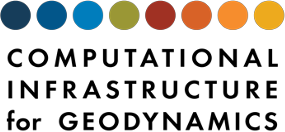
\includegraphics[scale=1.5]{../../logos/cig_logo_dots}%
  \hspace{4em}%
\raisebox{1em}{\includegraphics[scale=1.0]{../../logos/cig_short_pylith}}}
\date{June 21, 2022}


% ---------------------------------------------------- CUSTOMIZATION
\usetheme{CIG}
% Style information for PyLith presentations.

% Colors
\definecolor{ltorange}{rgb}{1.0, 0.74, 0.41} % 255/188/105
\definecolor{orange}{rgb}{0.96, 0.50, 0.0} % 246/127/0

\definecolor{ltred}{rgb}{1.0, 0.25, 0.25} % 255/64/64
\definecolor{red}{rgb}{0.79, 0.00, 0.01} % 201/0/3

\definecolor{ltpurple}{rgb}{0.81, 0.57, 1.00} % 206/145/255
\definecolor{purple}{rgb}{0.38, 0.00, 0.68} % 97/1/175

\definecolor{ltblue}{rgb}{0.2, 0.73, 1.0} % 51/187/255
\definecolor{mdblue}{rgb}{0.28, 0.50, 0.80} % 72/128/205
\definecolor{blue}{rgb}{0.12, 0.43, 0.59} % 30/110/150

\definecolor{ltltgreen}{rgb}{0.7, 1.00, 0.7} % 96/204/14
\definecolor{ltgreen}{rgb}{0.37, 0.80, 0.05} % 96/204/14
\definecolor{green}{rgb}{0.23, 0.49, 0.03} % 59/125/8
  
\definecolor{dkslate}{rgb}{0.18, 0.21, 0.28} % 47/53/72
\definecolor{mdslate}{rgb}{0.45, 0.50, 0.68} % 114/127/173
\definecolor{ltslate}{rgb}{0.85, 0.88, 0.95} % 216/225/229


\newcommand{\includefigure}[2][]{{\centering\includegraphics[#1]{#2}\par}}
\newcommand{\highlight}[1]{{\bf\usebeamercolor[fg]{structure}#1}}
\newcommand{\important}[1]{{\color{red}#1}}
\newcommand{\issue}[2]{\item[Issue:] {\color{red}#1}\\{\item[Soln:] \color{blue}#2}\\[4pt]}

\setbeamercolor{alerted text}{fg=ltgreen}
\setbeamertemplate{description item}[align left]


\newcommand{\lhs}[1]{{\color{blue}#1}}
\newcommand{\rhs}[1]{{\color{red}#1}}
\newcommand{\annotateL}[2]{%
  {\color{blue}\underbrace{\color{blue}#1}_{\color{blue}\mathclap{#2}}}}
\newcommand{\annotateR}[2]{%
  {\color{red}\underbrace{\color{red}#1}_{\color{red}\mathclap{#2}}}}
\newcommand{\eqnannotate}[2]{%
  {\color{blue}%
  \underbrace{\color{black}#1}_{\color{blue}\mathclap{#2}}}}

\newcommand{\trialvec}[1][]{{\vec{\psi}_\mathit{trial}^{#1}}}
\newcommand{\trialscalar}[1][]{{\psi_\mathit{trial}^{#1}}}
\newcommand{\basisvec}[1][]{{\vec{\psi}_\mathit{basis}^{#1}}}
\newcommand{\basisscalar}[1][]{{\psi_\mathit{basis}^{#1}}}

\newcommand{\tensor}[1]{\bm{#1}}
\DeclareMathOperator{\Tr}{Tr}

\usefonttheme[onlymath]{serif}

% minted shortcuts
\newminted{cfg}{bgcolor=ltslate,autogobble,fontsize=\tiny}
\newminted{bash}{bgcolor=ltltgreen,autogobble,fontsize=\tiny}

% PyLith components
\newcommand{\pylith}[1]{{\ttfamily\color{magenta}#1}}



% ========================================================= DOCUMENT
\begin{document}

% ------------------------------------------------------------ SLIDE
\maketitle

\logo{\includegraphics[height=4.5ex]{../../logos/cig_short_pylith}}

% ========================================================== SECTION
\section{{\ttfamily examples/strikeslip-2d}}

% ========================================================== SUBSECTION
\subsection{Overview}

% ------------------------------------------------------------ SLIDE
\begin{frame}
  \frametitle{Horizontal Cross-Section of Strike-Slip Fault (2D)}
  \summary{}

  \includefigure[height=6.1cm]{figs/geometry}

  \vfill
  Solve the static and quasistatic boundary elasticity equation for a horizontal cross-section of a strike-slip fault.
  
\end{frame}


% ------------------------------------------------------------ SLIDE
\begin{frame}
  \frametitle{Steps in example}
  \summary{}

  \begin{description}
    \item[Step 1] Static coseismic slip with Dirichlet (displacement) boundary conditions.
    \item[Step 2] Quasistatic coseismic slip with time-dependent Dirichlet (displacement) boundary conditions.
    \item[Step 3] Quasistatic slip with two ruptures and time-dependent Dirichlet (displacement) boundary conditions.
    \item[Step 4] \highlight{Variable slip and Dirichlet (displacement) boundary conditions.}
    \item[Step 5] \highlight{Static Green’s functions with Dirichlet (displacement) boundary conditions.}
    \item[Step 6] \highlight{Invert for slip in Step 4 using Green’s functions from Step 5.}
  \end{description}
  
\end{frame}


% ------------------------------------------------------------ SLIDE
\begin{frame}
  \frametitle{Concepts covered}
  \summary{}

  \begin{itemize}
  \item Generation of simple mesh using Gmsh
  \item Generation of randomly located synthetic GPS stations using \python{numpy}
  \item Simulation of a coseismic event in 2D
  \item Generation of static Green's functions
  \item Simple inversion of synthetic data using \python{numpy}
  \item Plotting of inversion results using \python{matplotlib} and \python{h5py}
  \end{itemize}
  
\end{frame}

% ========================================================== SUBSECTION
\subsection{Finite-Element Mesh}

% ------------------------------------------------------------ SLIDE
\begin{frame}
  \frametitle{Geometry}
  \summary{}

  We construct the geometry by first creating points, then connecting the points into curves, and finally the curves into surfaces.
  
  \includefigure[height=7.0cm]{figs/geometry-gmsh}
  
\end{frame}


% ------------------------------------------------------------ SLIDE
\begin{frame}
  \frametitle{Creating the finite-element mesh}
  \summary{}

  \begin{onlyenv}<1>
    \begin{itemize}
    \item Each curve in Gmsh has a direction (orientation).
    \item The direction is from the starting point to the ending point.
    \item When connecting curves into surfaces, you must connect the curves in a consistent direction.
    \item We connect the curves in a counter-clockwise direction.
    \item To reverse the direction of a curve, use the negative tag.
    \end{itemize}
  \end{onlyenv}
  \begin{onlyenv}<2>
  \includefigure[height=7.0cm]{figs/gmsh-tri}
  \end{onlyenv}
  
\end{frame}


% ========================================================== SECTION
\subsection{Files used for simulations}

% ------------------------------------------------------------ SLIDE
\begin{frame}
  \frametitle{Files used in simulations}
  \summary{Files are in directory {\tt examples/strikeslip-2d}}

  \begin{description}
  \item[README.md] Brief description of the various examples
  \item[*.cfg] PyLith parameter files
  \item[generate\_gmsh.py] Python script to generate mesh using Gmsh
  \item[generate\_gpsstations.py] Python script to generate synthetic
    GPS sites
  \item[invert\_slip.py] Python script to invert synthetic data for
    fault slip
  \item[*.msh] Finite-element mesh files generated by Gmsh
  \item[*.spatialdb] Spatial database files
  \item[viz] Directory containing ParaView Python scripts and other files for visualizing results
  \item[output] Directory containing simulation output; created automatically when running the simulations
  \end{description}

\end{frame}

% ========================================================== SUBSECTION
\subsection{Background}

% ------------------------------------------------------------ SLIDE
\begin{frame}
  \frametitle{Green's Functions}
  \summary{}

  \begin{itemize}
  \item Compute deformation due to unit (1 m) slip at fault vertices for use in an inversion for fault slip
    \begin{itemize}
    \item Slip decreases {\bf linearly} to 0 at surrounding vertices (basis order = 1)
    \item Similar but not equivalent to uniform slip over a patch (Okada dislocation)
    \item PyLith interpolates the responses to user-specified points using \pylith{OutputSolnPoints}
    \end{itemize}
  \item Provides ability to compute Green's functions with arbitrarily complex elastic structure and topography
  \end{itemize}
  
\end{frame}


% ========================================================== SECTION
\subsection{step04-varslip}

% ------------------------------------------------------------ SLIDE
\begin{frame}
  \frametitle{Step 4: Overview}
  \summary{Spatially variable coseismic slip with Dirichlet (displacement) boundary conditions}

  \includefigure[height=6.5cm]{figs/step04-diagram}
      
\end{frame}

% ------------------------------------------------------------ SLIDE
\begin{frame}
  \frametitle{Step 4: Physics}
  \summary{}

  \begin{minipage}{0.35\textwidth}
    {\scriptsize
    \begin{gather*}
    % Solution
    \vec{s}^T = \left( \vec{u} \quad \vec{\lambda} \right)^T \\
    % Elasticity
    \tensor{\nabla} \cdot \tensor{\sigma}(\vec{u}) = \vec{0} \\
    \rho_1, \mu_1, K_1 \text{ in elasticity\_xneg} \\ 
    \rho_2, \mu_2, K_2 \text{ in elasticity\_xpos} \\ 
    % Dirichlet
    \left. \begin{array}{c} u_x = 0 \\ u_y = 0 \end{array}\right\} \text{ on boundary\_xneg} \\
    \left. \begin{array}{c} u_x = 0 \\ u_y = 0 \end{array}\right\} \text{ on boundary\_xpos} \\
    % Prescribed slip
    d = d(y) \text{ on fault}
    \end{gather*}}
  \end{minipage}
  \hfill
  \begin{minipage}{0.60\textwidth}
    \includefigure[height=6.0cm]{figs/step04-diagram}
  \end{minipage}
      
\end{frame}


% ------------------------------------------------------------ SLIDE
\begin{frame}[t,fragile]
  \frametitle{Step 4: Physics to simulation parameters}
  \summary{}

  \begin{minipage}[t]{0.35\textwidth}
    {\scriptsize
    \begin{gather*}
    % Solution
    \vec{s}^T = \left( \vec{u} \quad \vec{\lambda} \right)^T \tikzmark{solution}\\
    % Elasticity
    \tensor{\nabla} \cdot \tensor{\sigma}(\vec{u}) = \vec{0} \tikzmark{material} \\
    \rho_1, \mu_1, K_1 \text{ in elasticity\_xneg} \\ 
    \rho_2, \mu_2, K_2 \text{ in elasticity\_xpos} \\ 
    % Dirichlet
    \left. \begin{array}{c} u_x = 0 \\ u_y = 0 \end{array}\right\} \text{ on boundary\_xpos} \tikzmark{bc}\\
    \left. \begin{array}{c} u_x = 0 \\ u_y = 0 \end{array}\right\} \text{ on boundary\_xneg} \\
    % Prescribed slip
    d = d(y) \text{ on fault} \tikzmark{fault}
    \end{gather*}}
  \end{minipage}
  \hfill
  \begin{minipage}[t]{0.60\textwidth}
    % Solution
    \begin{onlyenv}<2>
      \tikzmark{solution-cfg}
      \begin{cfgcode}
        [pylithapp.problem]
        solution = pylith.problems.SolnDispLagrange
        defaults.quadrature_order = 2
        
        [pylithapp.problem.solution.subfields]
        displacement.basis_order = 2
        lagrange_fault.basis_order = 2
      \end{cfgcode}
    \end{onlyenv}
    %
    % Governing equations
    \begin{onlyenv}<3>
      \tikzmark{material-cfg}
      \begin{cfgcode}
        [pylithapp.problem]
        materials = [elastic_xneg, elastic_xpos]

        [pylithapp.problem.materials.elastic_xneg]
        description = Material on the -x side of the fault
        label_value = 1

        db_auxiliary_field = spatialdata.spatialdb.UniformDB
        db_auxiliary_field.description = Elastic properties xneg
        db_auxiliary_field.values = [density, vs, vp]
        db_auxiliary_field.data = [2500.0*kg/m**3, 3.00*km/s, 5.29*km/s]

        auxiliary_subfields.density.basis_order = 0
        bulk_rheology.auxiliary_subfields.bulk_modulus.basis_order = 0
        bulk_rheology.auxiliary_subfields.shear_modulus.basis_order = 0

        derived_subfields.cauchy_strain.basis_order = 0
        derived_subfields.cauchy_stress.basis_order = 0

        [pylithapp.problem.materials.elastic_xneg]
        ...
      \end{cfgcode}
    \end{onlyenv}
    %
    % Boundary conditions
    \begin{onlyenv}<4>
      \tikzmark{bc-cfg}
      \begin{cfgcode}
        [pylithapp.problem]
        bc = [bc_xneg, bc_xpos]
        bc.bc_xneg = pylith.bc.DirichletTimeDependent
        bc.bc_xpos = pylith.bc.DirichletTimeDependent
        
        [pylithapp.problem.bc.bc_xpos]
        label = boundary_xpos
        label_value = 11
        constrained_dof = [0, 1]
        db_auxiliary_field = pylith.bc.ZeroDB
        db_auxiliary_field.description = Dirichlet BC +x boundary

        [pylithapp.problem.bc.bc_xpos]
        ...
      \end{cfgcode}
    \end{onlyenv}
    %
    % Fault
    \begin{onlyenv}<5>
      \tikzmark{fault-cfg}
      \begin{cfgcode}
        [pylithapp.problem]
        interfaces = [fault]

        [pylithapp.problem.interfaces.fault]
        label = fault
        label_value = 20

        [pylithapp.problem.interfaces.fault.eq_ruptures.rupture]
        db_auxiliary_field = spatialdata.spatialdb.SimpleDB
        db_auxiliary_field.description = Fault rupture auxiliary field spatial database
        db_auxiliary_field.iohandler.filename = slip_variable.spatialdb
      \end{cfgcode}
    \end{onlyenv}
  \end{minipage}

  \begin{tikzpicture}[overlay,remember picture]
    \draw[physics-arrow,visible on=<2>] ($(pic cs:solution-cfg)-(0,2em)$) to (pic cs:solution);
    \draw[physics-arrow,visible on=<3>] ($(pic cs:material-cfg)-(0,2em)$) to (pic cs:material);
    \draw[physics-arrow,visible on=<4>] ($(pic cs:bc-cfg)-(0,2em)$) to (pic cs:bc);
    \draw[physics-arrow,visible on=<5>] ($(pic cs:fault-cfg)-(0,2em)$) to (pic cs:fault);
  \end{tikzpicture}
  
\end{frame}


% ------------------------------------------------------------ SLIDE
\begin{frame}
  \frametitle{Step 4: Slip distribution}
  \summary{}

  \includefigure[width=\textwidth]{figs/step04-slip}
    
\end{frame}


% ------------------------------------------------------------ SLIDE
\begin{frame}
  \frametitle{Step 4: Input files}
  \summary{}

  \begin{description}
  \item[mesh\_tri.msh] Finite-element mesh generated using Gmsh
  \item[pylithapp.cfg] PyLith parameter file common to all steps
  \item[step04\_varslip.cfg] PyLith parameter file
  \item[slip\_variable.spatialdb] Spatial database for slip distribution
  \item[gps\_stations.txt] List of GPS stations (station code and coordinates)
  \end{description}
    
\end{frame}


% ------------------------------------------------------------ SLIDE
\begin{frame}[fragile]
  \frametitle{Step 4: Run the simulation}
  \summary{}

\begin{bashcode}
pylith step04_varslip.cfg

# Output
 >> /software/unix/py39-venv/pylith-debug/lib/python3.9/site-packages/pylith/meshio/MeshIOObj.py:44:read
 -- meshiopetsc(info)
 -- Reading finite-element mesh
 >> /src/cig/pylith/libsrc/pylith/meshio/MeshIO.cc:94:void pylith::meshio::MeshIO::read(topology::Mesh *)
 -- meshiopetsc(info)
 -- Component 'reader': Domain bounding box:
    (-50000, 50000)
    (-75000, 75000)

# -- many lines omitted --

 -- Solving problem.
0 TS dt 0.01 time 0.
    0 SNES Function norm 3.840123479624e-03
    Linear solve converged due to CONVERGED_ATOL iterations 73
    1 SNES Function norm 2.286140232631e-12
  Nonlinear solve converged due to CONVERGED_FNORM_ABS iterations 1
1 TS dt 0.01 time 0.01
 >> /software/unix/py39-venv/pylith-debug/lib/python3.9/site-packages/pylith/problems/Problem.py:201:finalize
 -- timedependent(info)
 -- Finalizing problem.
\end{bashcode}
  
\end{frame}


% ------------------------------------------------------------ SLIDE
\begin{frame}
  \frametitle{Step 4: Visualize results}
  \summary{Run the {\tt viz/plot\_dispwarp.py} Python script from within ParaView}

  \includefigure[height=7.0cm]{figs/step04-solution}
    
\end{frame}


% ========================================================== SECTION
\subsection{step05-greensfns}

% ------------------------------------------------------------ SLIDE
\begin{frame}
  \frametitle{Step 5: Overview}
  \summary{Compute response to static fault slip impulses}

  \includefigure[height=6.5cm]{figs/step05-diagram}
      
\end{frame}

% ------------------------------------------------------------ SLIDE
\begin{frame}
  \frametitle{Step 5: Physics}
  \summary{}

  \begin{minipage}{0.35\textwidth}
    {\scriptsize
    \begin{gather*}
    % Solution
    \vec{s}^T = \left( \vec{u} \quad \vec{\lambda} \right)^T \\
    % Elasticity
    \tensor{\nabla} \cdot \tensor{\sigma}(\vec{u}) = \vec{0} \\
    \rho_1, \mu_1, K_1 \text{ in elasticity\_xneg} \\ 
    \rho_2, \mu_2, K_2 \text{ in elasticity\_xpos} \\ 
    % Dirichlet
    \left. \begin{array}{c} u_x = 0 \\ u_y = 0 \end{array}\right\} \text{ on boundary\_xneg} \\
    \left. \begin{array}{c} u_x = 0 \\ u_y = 0 \end{array}\right\} \text{ on boundary\_xpos} \\
    % Prescribed slip
    d = \delta(y) \text{ on fault}
    \end{gather*}}
  \end{minipage}
  \hfill
  \begin{minipage}{0.60\textwidth}
    \includefigure[height=6.0cm]{figs/step05-diagram}
  \end{minipage}
      
\end{frame}


% ------------------------------------------------------------ SLIDE
\begin{frame}[t,fragile]
  \frametitle{Step 5: Physics to simulation parameters}
  \summary{}

  \begin{minipage}[t]{0.35\textwidth}
    {\scriptsize
    \begin{gather*}
    % Solution
    \vec{s}^T = \left( \vec{u} \quad \vec{\lambda} \right)^T \tikzmark{solution}\\
    % Elasticity
    \tensor{\nabla} \cdot \tensor{\sigma}(\vec{u}) = \vec{0} \tikzmark{material} \\
    \rho_1, \mu_1, K_1 \text{ in elasticity\_xneg} \\ 
    \rho_2, \mu_2, K_2 \text{ in elasticity\_xpos} \\ 
    % Dirichlet
    \left. \begin{array}{c} u_x = 0 \\ u_y = 0 \end{array}\right\} \text{ on boundary\_xpos} \tikzmark{bc}\\
    \left. \begin{array}{c} u_x = 0 \\ u_y = 0 \end{array}\right\} \text{ on boundary\_xneg} \\
    % Prescribed slip
    d = \delta(y) \text{ on fault} \tikzmark{fault}
    \end{gather*}}
  \end{minipage}
  \hfill
  \begin{minipage}[t]{0.60\textwidth}
    % Problem and solution
    \begin{onlyenv}<2>
      \tikzmark{solution-cfg}
      \begin{cfgcode}
        [pylithapp]
        problem = pylith.problems.GreensFns

        [pylithapp.greensfns]
        label = fault
        label_value = 20

        solution = pylith.problems.SolnDispLagrange
        defaults.quadrature_order = 1
        
        [pylithapp.problem.solution.subfields]
        displacement.basis_order = 1
        lagrange_fault.basis_order = 1
      \end{cfgcode}
    \end{onlyenv}
    %
    % Governing equations
    \begin{onlyenv}<3>
      \tikzmark{material-cfg}
      \begin{cfgcode}
        # Same for all simulations in directory
      \end{cfgcode}
    \end{onlyenv}
    %
    % Boundary conditions
    \begin{onlyenv}<4>
      \tikzmark{bc-cfg}
      \begin{cfgcode}
        # Same for all simulations in directory
      \end{cfgcode}
    \end{onlyenv}
    %
    % Fault
    \begin{onlyenv}<5>
      \tikzmark{fault-cfg}
      \begin{cfgcode}
        [pylithapp.problem.interfaces]
        fault = pylith.faults.FaultCohesiveImpulses

        [pylithapp.problem.interfaces.fault]
        impulse_dof = [1]

        db_auxiliary_field = spatialdata.spatialdb.SimpleDB
        db_auxiliary_field.description = Fault rupture auxiliary field spatial database
        db_auxiliary_field.iohandler.filename = slip_impulses.spatialdb

        auxiliary_subfields.slip.basis_order = 1
      \end{cfgcode}
    \end{onlyenv}
  \end{minipage}

  \begin{tikzpicture}[overlay,remember picture]
    \draw[physics-arrow,visible on=<2>] ($(pic cs:solution-cfg)-(0,2em)$) to (pic cs:solution);
    \draw[physics-arrow,visible on=<3>] ($(pic cs:material-cfg)-(0,2em)$) to (pic cs:material);
    \draw[physics-arrow,visible on=<4>] ($(pic cs:bc-cfg)-(0,2em)$) to (pic cs:bc);
    \draw[physics-arrow,visible on=<5>] ($(pic cs:fault-cfg)-(0,2em)$) to (pic cs:fault);
  \end{tikzpicture}
  
\end{frame}


% ------------------------------------------------------------ SLIDE
\begin{frame}
  \frametitle{Step 5: Input files}
  \summary{}

  \begin{description}
  \item[mesh\_tri.msh] Finite-element mesh generated using Gmsh
  \item[pylithapp.cfg] PyLith parameter file common to all steps
  \item[step05\_greensfns.cfg] PyLith parameter file
  \item[slip\_impulses.spatialdb] Spatial database for slip distribution
  \item[gps\_stations.txt] List of GPS stations (station code and coordinates)
  \end{description}
    
\end{frame}


% ------------------------------------------------------------ SLIDE
\begin{frame}[fragile]
  \frametitle{Step 5: Run the simulation}
  \summary{}

\begin{bashcode}
pylith step05_greensfns.cfg

# Output
# -- many lines omitted --

 -- Component 'problem': Computing Green's function 12 of 12.
  0 SNES Function norm 3.027654014252e-03
  Linear solve converged due to CONVERGED_ATOL iterations 46
  1 SNES Function norm 2.204080482014e-12
Nonlinear solve converged due to CONVERGED_ITS iterations 1
 >> /software/unix/py39-venv/pylith-debug/lib/python3.9/site-packages/pylith/problems/Problem.py:201:finalize
 -- greensfns(info)
 -- Finalizing problem.
WARNING! There are options you set that were not used!
WARNING! could be spelling mistake, etc!
There are 3 unused database options. They are:
Option left: name:-ts_error_if_step_fails (no value)
Option left: name:-ts_monitor (no value)
Option left: name:-ts_type value: beuler
\end{bashcode}
  
\end{frame}


% ------------------------------------------------------------ SLIDE
\begin{frame}
  \frametitle{Step 5: Visualize results}
  \summary{Run the {\tt viz/plot\_dispwarp.py} Python script from within ParaView}

  \includefigure[height=7.0cm]{figs/step05-solution}
    
\end{frame}


% ========================================================== SECTION
\subsection{step06-inversion}

% ------------------------------------------------------------ SLIDE
\begin{frame}
  \frametitle{Step 6: Overview}
  \summary{}

  Invert for fault slip in Step 4 using Green's functions computed in Step 5.
      
\end{frame}


% ------------------------------------------------------------ SLIDE
\begin{frame}
  \frametitle{Simple Linear Inversion Parameters}
  \summary{}

  \begin{description}
  \item[$G$] Green's function matrix
  \item[$d$] Unknown fault slip
  \item[$d_\mathit{apriori}$] A priori estimate of fault slip
  \item[$u_\mathit{obs}$] Observed displacement
  \item[$D$] Penalty matrix
  \item[$\theta$] Penalty parameter
  \end{description}
  
  \vfill
  The matrix $G_{ij}$ gives displacement component $i$ due to a unit of slip from component $j$.

\end{frame}


% ------------------------------------------------------------ SLIDE
\begin{frame}
  \frametitle{Simple Linear Inversion Equations}
  \summary{}

  \begin{itemize}
  \item Original system of equations:
    \begin{equation}
      G d = u_\mathit{obs}
    \end{equation}
  \item Augmented system of equations:
    \begin{equation}
      G_a d = u_a \text{, where } 
      G_a = \left[ \begin{array}{c} G \\ \theta D \end{array} \right]
      \text{ and }
      u_a = \left[ \begin{array}{c} u_{obs} \\ d_\mathit{apriori} \end{array} \right]
    \end{equation}
  \item Generalized inverse:
    \begin{gather}
      G^{-g} = \left( G_a^T G_a \right)^{-1} G_a^T \\
      d_{est} = G^{-g} u_a
    \end{gather}
  \end{itemize}
  
\end{frame}


% ------------------------------------------------------------ SLIDE
\begin{frame}
  \frametitle{Step 6: Visualize results}
  \summary{Run the {\tt viz/plot\_inversion\_results.py} Python script from the command line}

  \includefigure[width=\textwidth]{figs/step06-solution}
  
\end{frame}

% ======================================================================
\end{document}


% End of file
